\chapter{Evaluierung}

Die Qualität der Ergebnisse des in der Implementierung realisierten Modells wird in diesem Kapitel durch ein Testexperiment überprüft. Weiterhin werden Ausführungszeiten für beispielsweise verschieden große $k$ beim Bag of Visual Words betrachtet, um eine Einsicht in die Performance der Algorithmen zu gewinnen.
Im Kapitel Experimentaufbau wird zunächst das Experiement sowie verwendete Metriken und Ergebnistypen behandelt. Nachfolgend wird erläutert, wie die großen Menge an benötigten Trainings- und Testdaten wiederholbar und automatisiert aufgebaut wird. Dieser Abschnitt illustriert auch, wie eine Durchführung des Experiments vonstattengeht. Im letzten Teil werden dann konkrete Testgruppen aus den Caltech101 \cite{cal2004} Bilddaten erzeugt. Diese Menge an Bilddaten hat große Verbreitung im Bereich der Objekterkennung gefunden. Auf diese Weise ist ein Vergleich mit Arbeiten Anderer prinzipiell möglich.

\section{Experimentaufbau}

Das Experiment soll zeigen, wie gut der jeweilige Algorithmus geeignet ist, um unüberwacht die Ähnlichkeit zwischen zwei Bildern zu beurteilen. \todo{Wie wird das Ergebnis bewertet? Distanzmetrik Histogramme}. Anhand einer Distanzmetrik kann dann die Ähnlichkeit der Histogramme bestimmt werden. Hier gibt es zwei Fälle zu unterscheiden:

\begin{itemize}
	\item \textbf{True Positives} Bei \textit{True Positives} handelt es sich um zwei Bildern die entweder in der gleichen oder einer verschiedenen Klasse liegen und die Vorhersage des Modells diesbezüglich korrekt ist.
	\item \textbf{False Positives} Auch hier liegen die Testbilder in der gleichen oder einer verschiedenen Klasse, die Vorhersage durch das Modell ist jedoch nicht korrekt.
\end{itemize}

Damit ein Modell zuverlässige Ergebnisse liefert, muss es größtenteils \textit{True Positives} erkennen, bzw. der Anteil der \textit{True Positives} sollte im Verhältnis zu den \textit{False Positives} bei weitem überwiegen. Für eine visuelle Darstellung dieses Verhältnisses eignet sich die \textit{Receiver Operating Characteristic (ROC)}: Diese stellt für verschiedene Parameter die \textit{True Positives} auf der Ordinate und die \textit{False-Positives} auf der Abzisse dar, sodass der optimale Parameter anhand der resultierenden Kurve abgelesen werden kann.

\section{Testdaten und Testgenerierung}

Der Abschnitt Testdaten stellt die hier verwendete Menge von Bildern vor, die Caltech101, welche extra für den Test von Algorithmen bezüglich der Objekterkennung in Bildern entwickelt wurde.\newline
Im Folgenden Abschnitt zur Testgenerierung wird ein Verfahren zur zufälligen Auswahl von Trainings- und Testbildern unter Berücksichtigung verschiedener Restriktionen, wie z.B. dem Verhältnis der Anzahl von Trainings- zu Testbildern vorgestellt.

\subsection{Testdaten}

Als Testmenge wurden die Bilder der Caltech101 Menge verwendet. Bei Caltech101 handelt es sich um eine weit verbreitete Menge von Bilddaten, die vorwiegend zum Test von Algorithmen bezüglich der Objekterkennung in Bildern dient. Insgesamt liegen, wie der Name sagt, 101 Kategorien vor, die jeweils zwischen 40 und 800 Bildern enthalten. Auf der offiziellen Webseite \footnote{http://www.vision.caltech.edu/Image\textunderscore Datasets/Caltech101/} und im Artikel der Autoren wir empfohlen, die eigene Arbeit mit derer anderen vergleichbar zu halten, indem:

\begin{itemize}
	\item Eine feste Anzahl an Trainings- und Testbildern verwendet wird.
	\item Experimente mit einer zufälligen Auswahl an Bildern wiederholt werden.
	\item Ähnlich viele Bilder, wie in den Arbeiten anderer, verwendet werden (1, 3, 5, 10, 15, 20 oder 30 Trainingsbilder; 20 oder 30 Testbilder).
\end{itemize}

Abbildung \ref{img:strawberries} zeigt vier Bilder aus der Kategorie \enquote{Erdbeere}. Neben Bildern von realen Rosengewächsen sind auch Zeichnungen und Objekte enthalten, die Form und Farbe der Erdbeere nachempfunden sind. 
Da der Bedarf nach bereits kategorisierten Testdaten unentwegt steigt, gibt es inzwischen eine Caltech250 Bildmenge, die für größere Experimente verwendet wird.

\begin{figure}
	\centering
	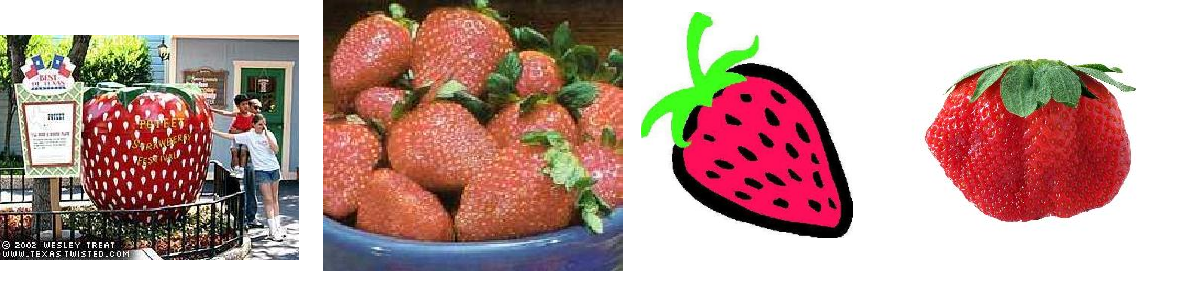
\includegraphics[scale=0.5]{images/strawberry.png}
	\caption{Verschiedene Bilder aus der Kategorie \enquote{Erdbeere} der Caltech101 Bilddaten.}
	\label{img:strawberries}
\end{figure}

\subsection{Testgenerierung}

Um durch die ROC-Kurve ein aussagekräftiges Ergebnis zu erhalten, muss eine große Anzahl an Bildern durch das Modell gegenübergestellt werden. Da hier mehr als 2000 Bildpaare verwendet werden sollen, wäre ein manueller Testaufbau mühsam und fehleranfällig. Aus diesem Grund wird dieser Prozess hier durch ein Programm automatisiert: Es werden zufällige Bildpaare ausgewählt und deren absolute Pfade, sowie die Information, ob die Bilder in der selben Klasse liegen gespeichert (\enquote{-} für verschiedene Klassen, \enquote{+} für dieselbe Klasse). Zwei Bilder liegen dabei in der selben Klasse, wenn sie im selben Ordner im Dateisystem enthalten sind. Die zu verwendenden Ordner (also Klassen), die Anzahl der zufällig zu generierenden Tests und das Verhältnis von gleichen zu verschiedenen Klassen muss bei der Erzeugung angegeben werden. Das Ergebnis wird dann als Datei \textit{test.txt} gespeichert, um wiederholt benutzbar zu sein.\newline
Im nächsten Schritt werden aus den ausgewählten Bildern die Features extrahiert und ebenfalls in einer Datei pro Bild gespeichert. Dieser Schritt ist leider erforderlich, da die Implementierung des Autoencoders in Python erfolgt ist und der nächste Schritt, das Clustering, in CUDA C. Die Features werden dabei im gleichen Ordner wie die Datei train.txt gespeichert und die Assoziation zum jeweiligen Bild wird über den Namen der Feature-Dateien hergestellt. Im Falle der Caltech101 Daten gelingt dies durch das Schema \textit{<categoryName>\textunderscore <imageName>.txt}.
Für jede werden nun die jeweiligen\textit{Visual Words} ermittelt und anhand der euklidischen Distanz verglichen. 

Nach dem alle Bilderpaare bewertet wurden, werden die Ergebnisse wieder in die Excel-Tabelle geschrieben und die ROC-Kurve durch eine Formel berechnet und in Excel visualisiert. Durch diesen Aufbau kann des Experiment immer mit einer großen, zufällig ausgewählten Menge an Bildern wiederholt werden.

\section{Experimentdurchführung}

\todo{LALALA}